\chapter{Applikationen und Webseite}
Die Applikationen und die Webseite sollen die Verwendung vom TIMA für möglichst
viele Endnutzer möglich machen.

\section{Webfrontend}
Das Webfrontend ist die Hauptanlaufstelle für Benutzer. Hierüber kann er sowohl anonym als auch angemeldet Assoziationen eingegeben, Wörter und
deren Assoziationen ansehen und weitere Funktionen wie die Rangliste und andere Statistiken aufrufen.

Das Webfrontend basiert auf Django, wurde zusätzlich zu HTML mit Bootstrap und JQuery erstellt, sowie zur Visualisierung D3.

\section{Applikation}
De Applikationen sollen die Verwendung von TIM ohne Webbrowser ermöglichen. Durch Applikationen wird besonders für mobile Geräte die Nutzung
vereinfacht.
In einer erste Variante der App wurden grundlegende Funktionen der
Webseite nachgebaut.  Dies diente auch der Entwicklung der API, um etwaige
Fehler im Protokoll oder Verbesserungen dessen aufzuzeigen und zu beheben.

\subsection{Framework}
Als Framework wurde sich für Qt5 entschieden Aufgrund der weitreichenden
Unterstützung des Frameworks auf verschiedenen Endgeräten. Hier ist besonders darauf hinzuweisen, das Qt5 sowohl auf Andriod als auch auf iOS läuft und so nicht die gleiche App für beide Betriebssysteme geschrieben werden muss.

\subsection{Aufbau}
Die innere Logik wird durch einen Zustandsautomaten dargestellt um
Mehrfachanfragen zu vermeiden und eine einfache Fehlerkorrektur zu ermöglichen.
In Abbildung \ref{fig:uml_automata} wird der Zusammenhang der einzelnen
Zustände angezeigt. Das wechseln der Zustände wird ausschließlich über die
Signale geregelt, die mit Qt implementiert sind.
\begin{figure}[!h]
	\centering
	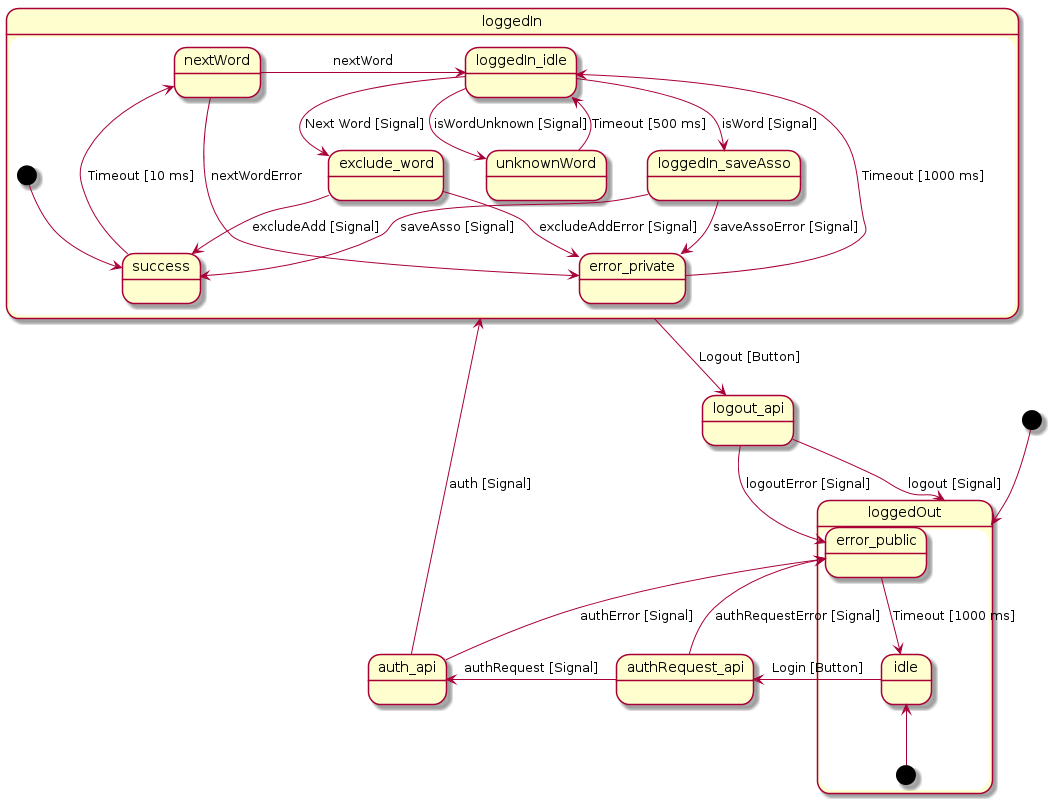
\includegraphics[width=\textwidth]{../UML/app_automata.png}
	\caption{UML State Diagramm des Applikationszustandsautomaten}
	\label{fig:uml_automata}
\end{figure}

\section{Sicherheit}
Die Sicherheit hat bei der Entwicklung eine große Rolle gespielt. Jede App und die Webseite nutzt die in \ref{subsec:autorisierte_anfragen} vorgestellte Autorisierungsmethode.  Dies dient dazu, lediglich von TIMA
akzeptierte Applikationen Schreibrechte für die Datenbank zu geben.  Das Auslesen
der Informationen bleibt davon jedoch unangetastet, sofern es sich nicht um benutzerspezifische Daten handelt, und ist nach wie vor für
jeden offen.
